\documentclass[10pt,oneside,a4paper]{article}
\usepackage[utf8]{inputenc}
\usepackage{amsmath}
\usepackage{indentfirst}
\usepackage{enumitem}
\usepackage[spanish]{babel}
\usepackage[export]{adjustbox}
\usepackage{graphicx}
\graphicspath{ {img/} }
\usepackage{listings}
\usepackage{subfig}
\usepackage{cite}

\addtolength{\oddsidemargin}{-.300in}
\addtolength{\evensidemargin}{-.300in}
\addtolength{\textwidth}{0.600in}
\addtolength{\topmargin}{-.300in}
\addtolength{\textheight}{0.600in} %1.75

\begin{document}
\begin{titlepage}

\title{\Huge Rendering Avanzado  \\[0.7in] \LARGE \textit{Path Tracing\\Entrega Final}\\[3.6in]}
\date{}
\author{Álvaro Muñoz Fernández\\
Iván Velasco González}
\maketitle
\thispagestyle{empty}
\end{titlepage}

\section{Introducción}
Para esta entrega debían añadirse al \emph{Path Tracer} desarrollado durante la asignatura un conjunto de funcionalidades adicionales que se emplearían para realizar un render basado en una imagen motivacional. En nuestro caso hemos optado por las funcionalidades de \emph{Depth of Field} y \emph{Environment Map Lighting}. Como imagen motivacional hemos seleccionado una imagen que creemos que es capaz de mostrar las capacidades de un \emph{Path Tracer}, y especialmente las funcionalidades que hemos implementado y que se ven representadas en dicha imagen.

\begin{figure}[h]
\centering
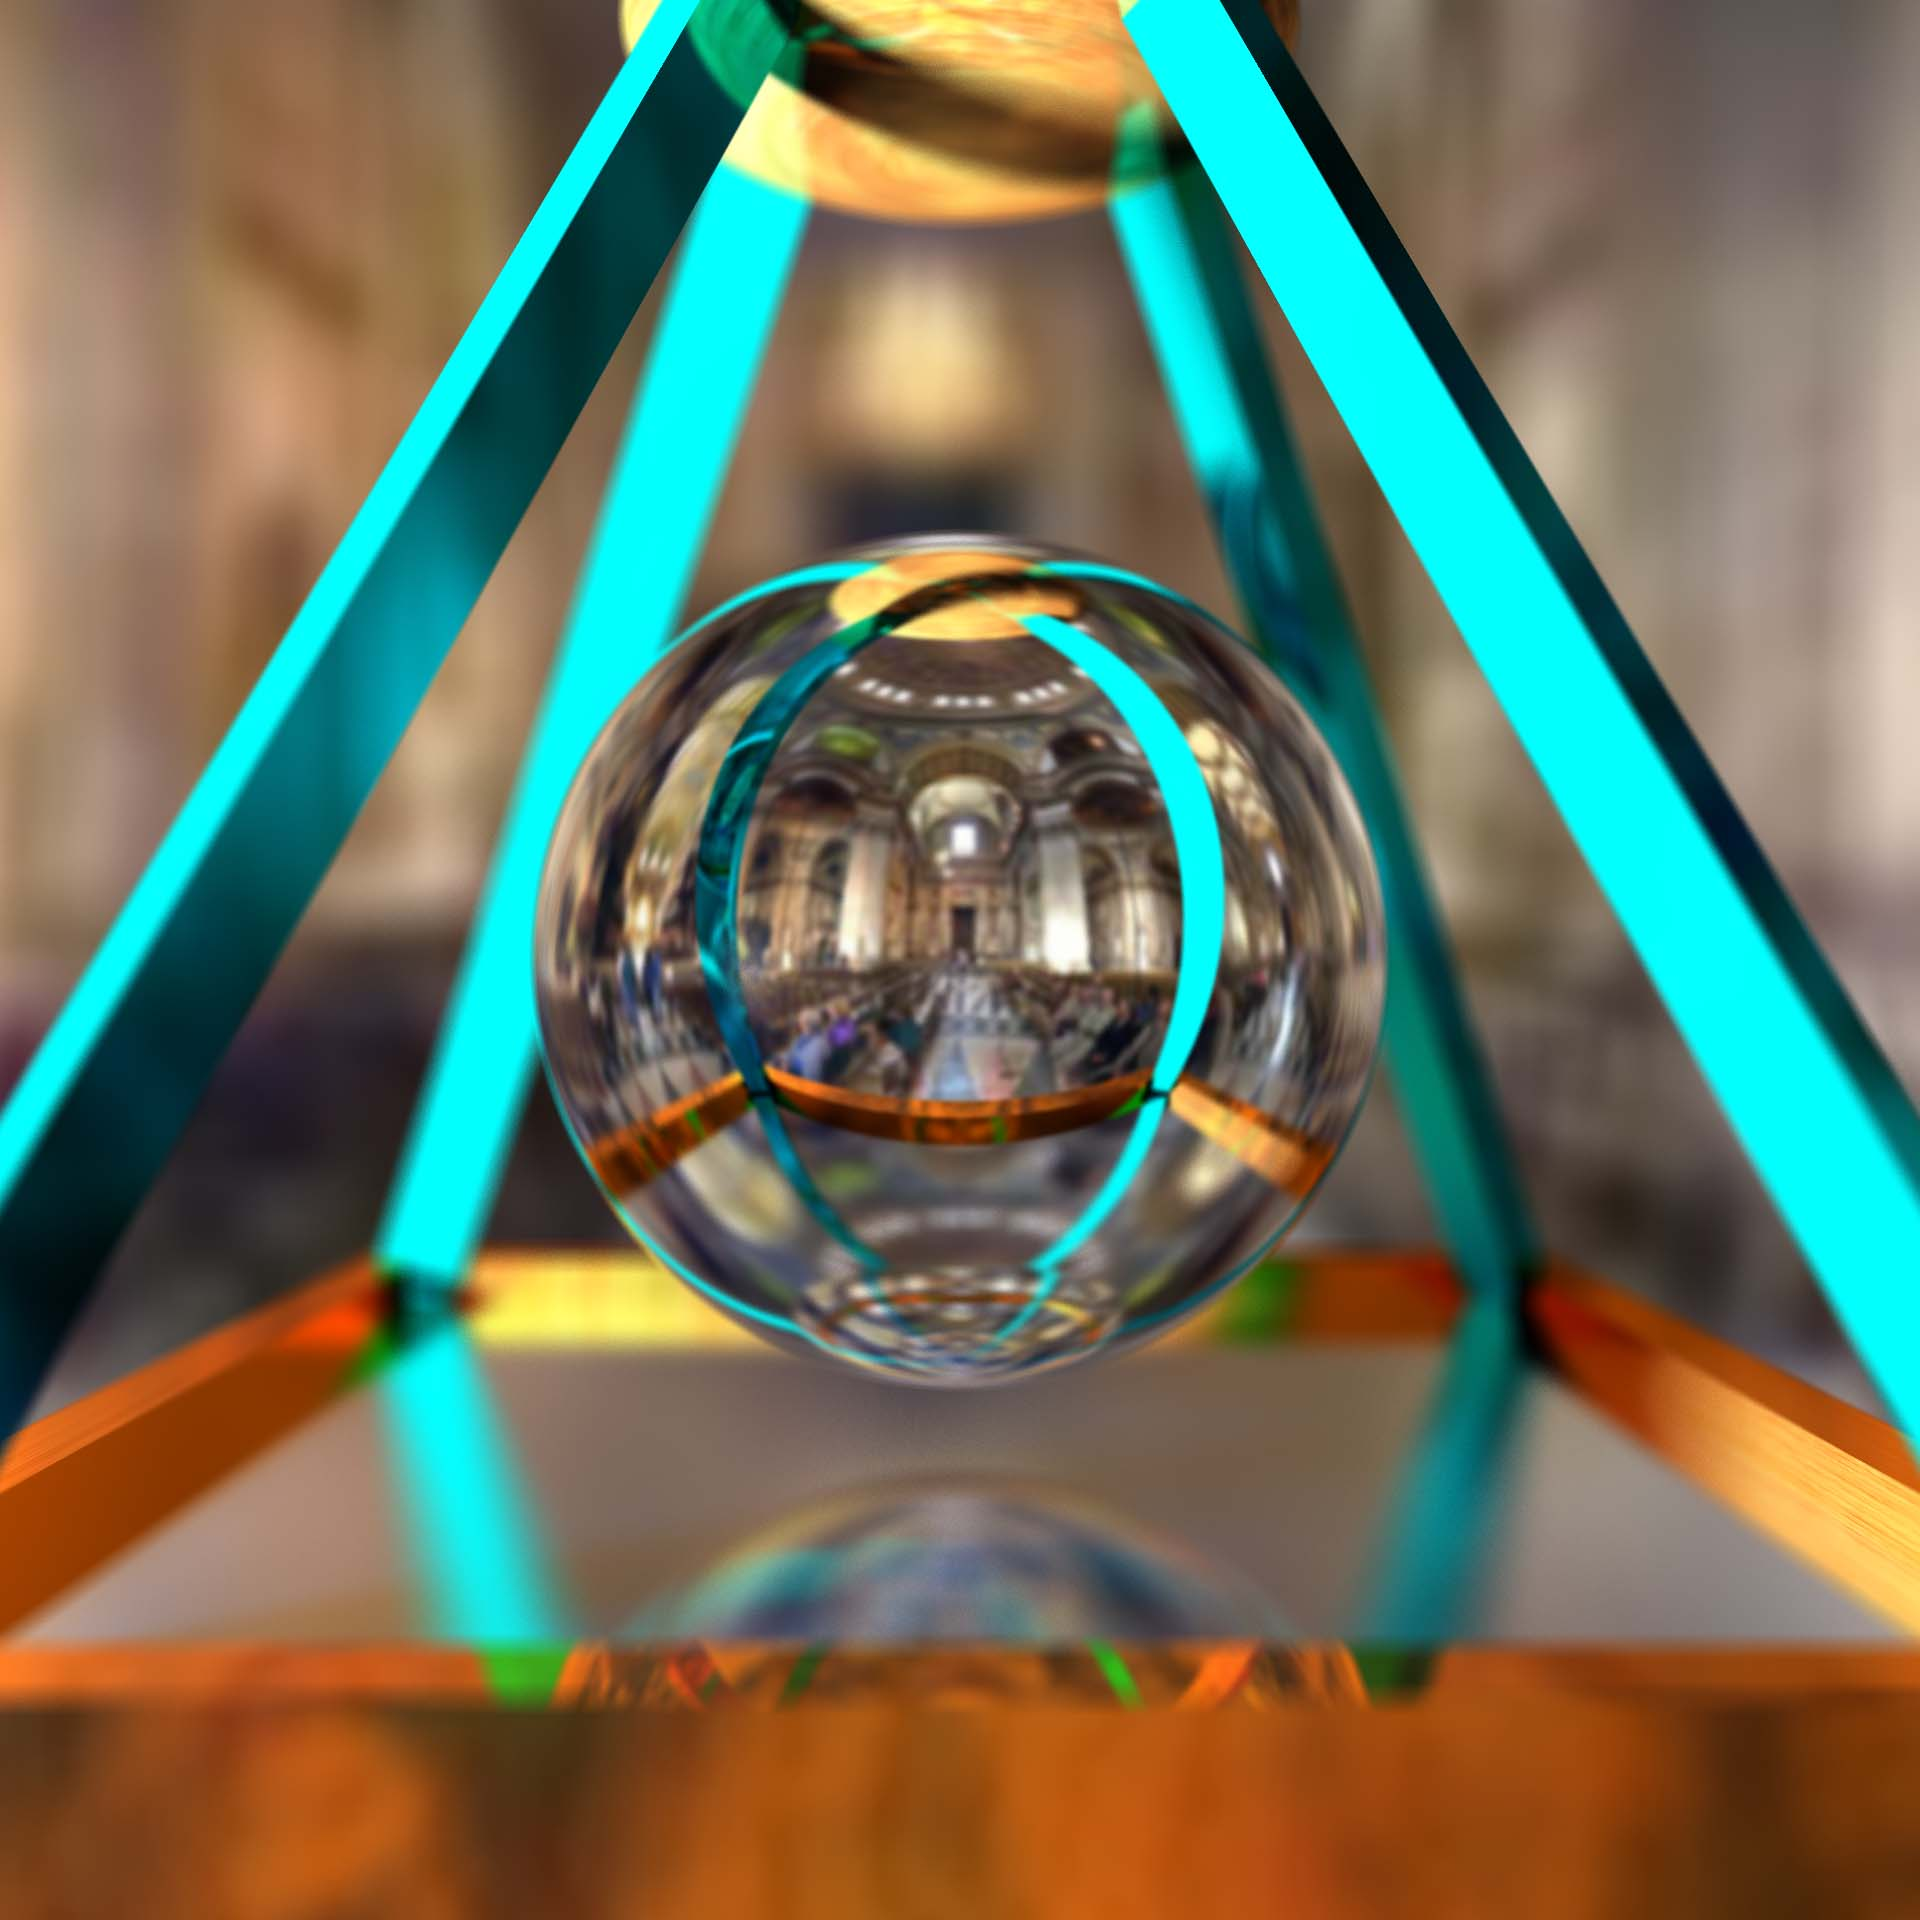
\includegraphics[width=1\linewidth]{images/motivacional.jpg}
\caption{Imagen motivacional sobre la que se basa nuestra entrega}
\label{fig:disp}
\end{figure}
\newpage

\section{Depth of Field}

\begin{figure}[h]
\centering
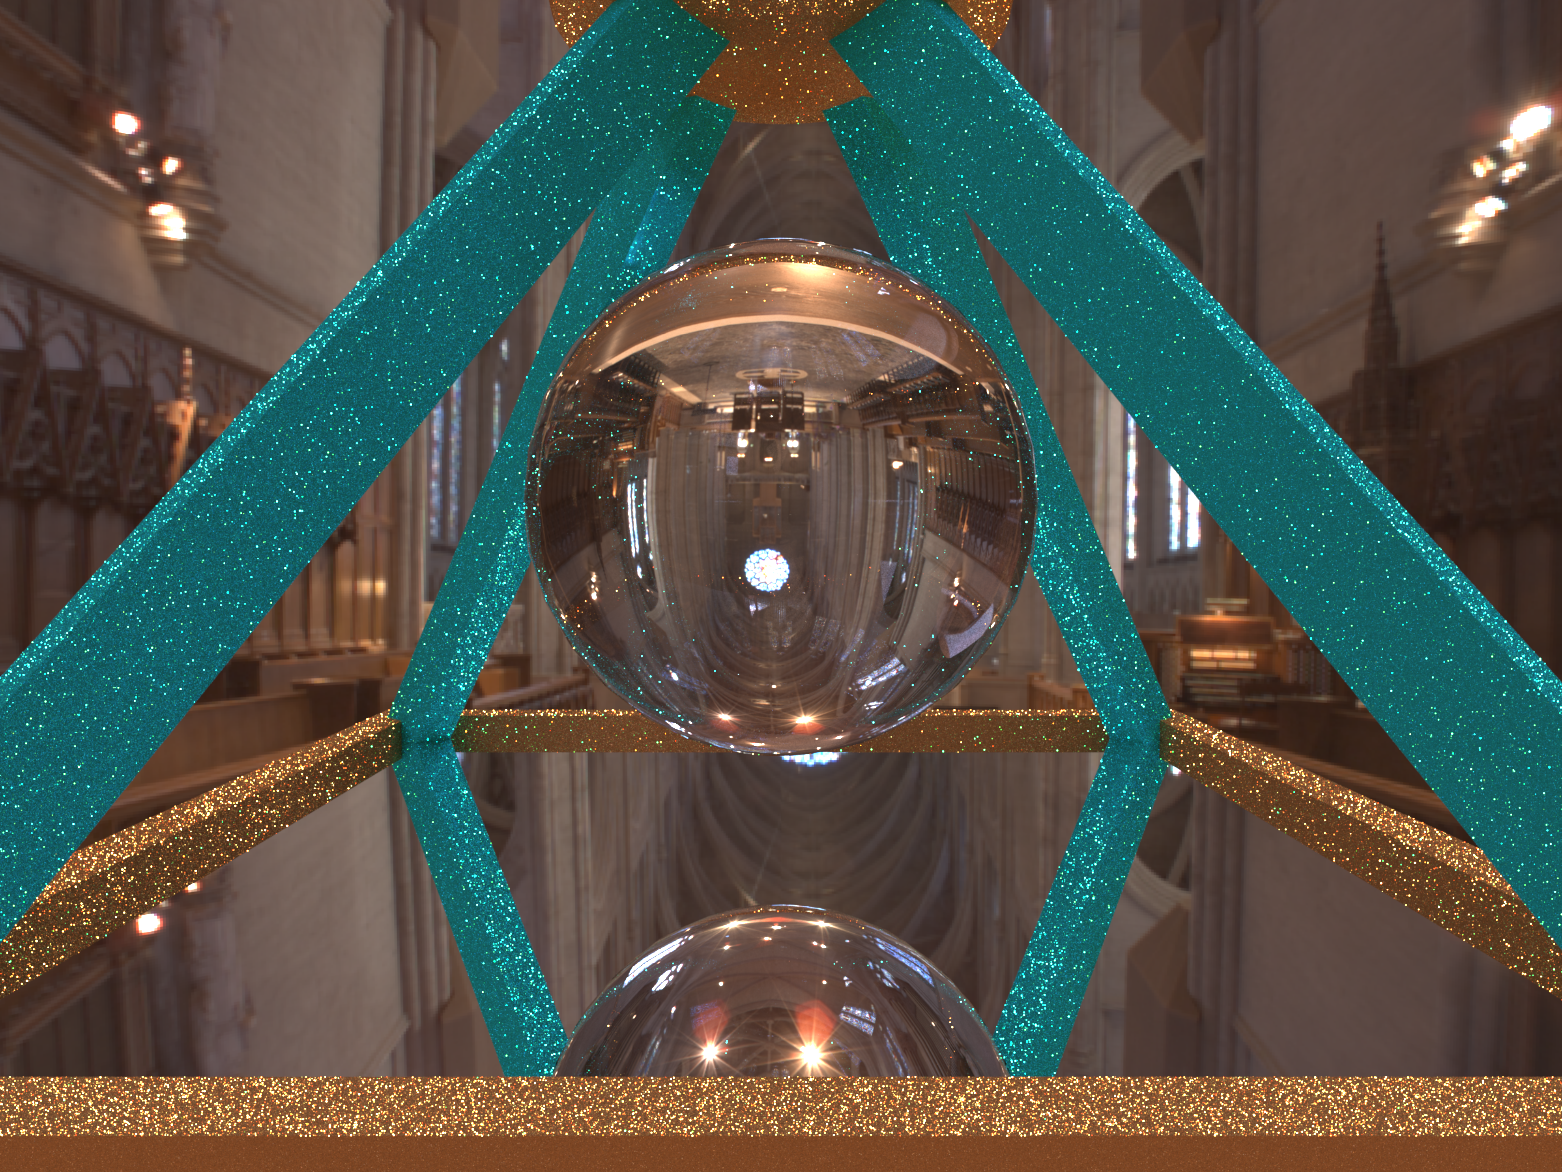
\includegraphics[width=1\linewidth]{images/escena_2400x1800_128spp_dof0-0_screencap.png}
\caption{Render sin DoF}
\label{fig:disp}
\end{figure}

Para implementar el \textit{Depth of Field} hemos creado una nueva cámara que sigue una aproximación de lente "delgada" (\textit{thin lens}), en la que solamente existe una lente y el grosor de esta es pequeño en relación a su radio. Para ello se va a incluir el efecto que produciría esta lente a la hora de muestrear un nuevo rayo desde la cámara.\\

En primer lugar, muestreamos de manera aleatoria un punto en la lente que será utilizado como origen del nuevo rayo. Para hacerlo muestreamos de manera uniforme un disco de radio 1 y multiplicamos el resultado por el radio elegido para la lente en cuestión. A continuación se obtiene el punto de enfoque el cual pertenece al plano de enfoque, los puntos de la escena que no se encuentren en este plano corresponderan con mas de un punto en el plano de imagén, llamado circulo de confusión, siendo su tamaño mayor mientras mas lejos se encuentre el punto del plano de enfoque ,mientras que para los puntos de la escena que se encuentren en el plano de enfoque no presentan circulo de confusión y un punto en la escena se corresponde con un unico punto en el plano de imagen. Para  obtener este punto de enfoque es necesario determinar la distancia siguiendo el rayo sin perturbar hasta el plano de enfoque, es decir, el plano donde no existe circulo de confusión y,por tanto,  un punto en la escena que corresponde con un punto en el plano de imagen. Esta distancia se obtiene mediante la operación $focalDistance/ ray\_dir.z$, y con este dato obtenemos el punto de enfoque desplazándonos esa distancia por el rayo.\\

%\begin{figure}[h]
%\centering
%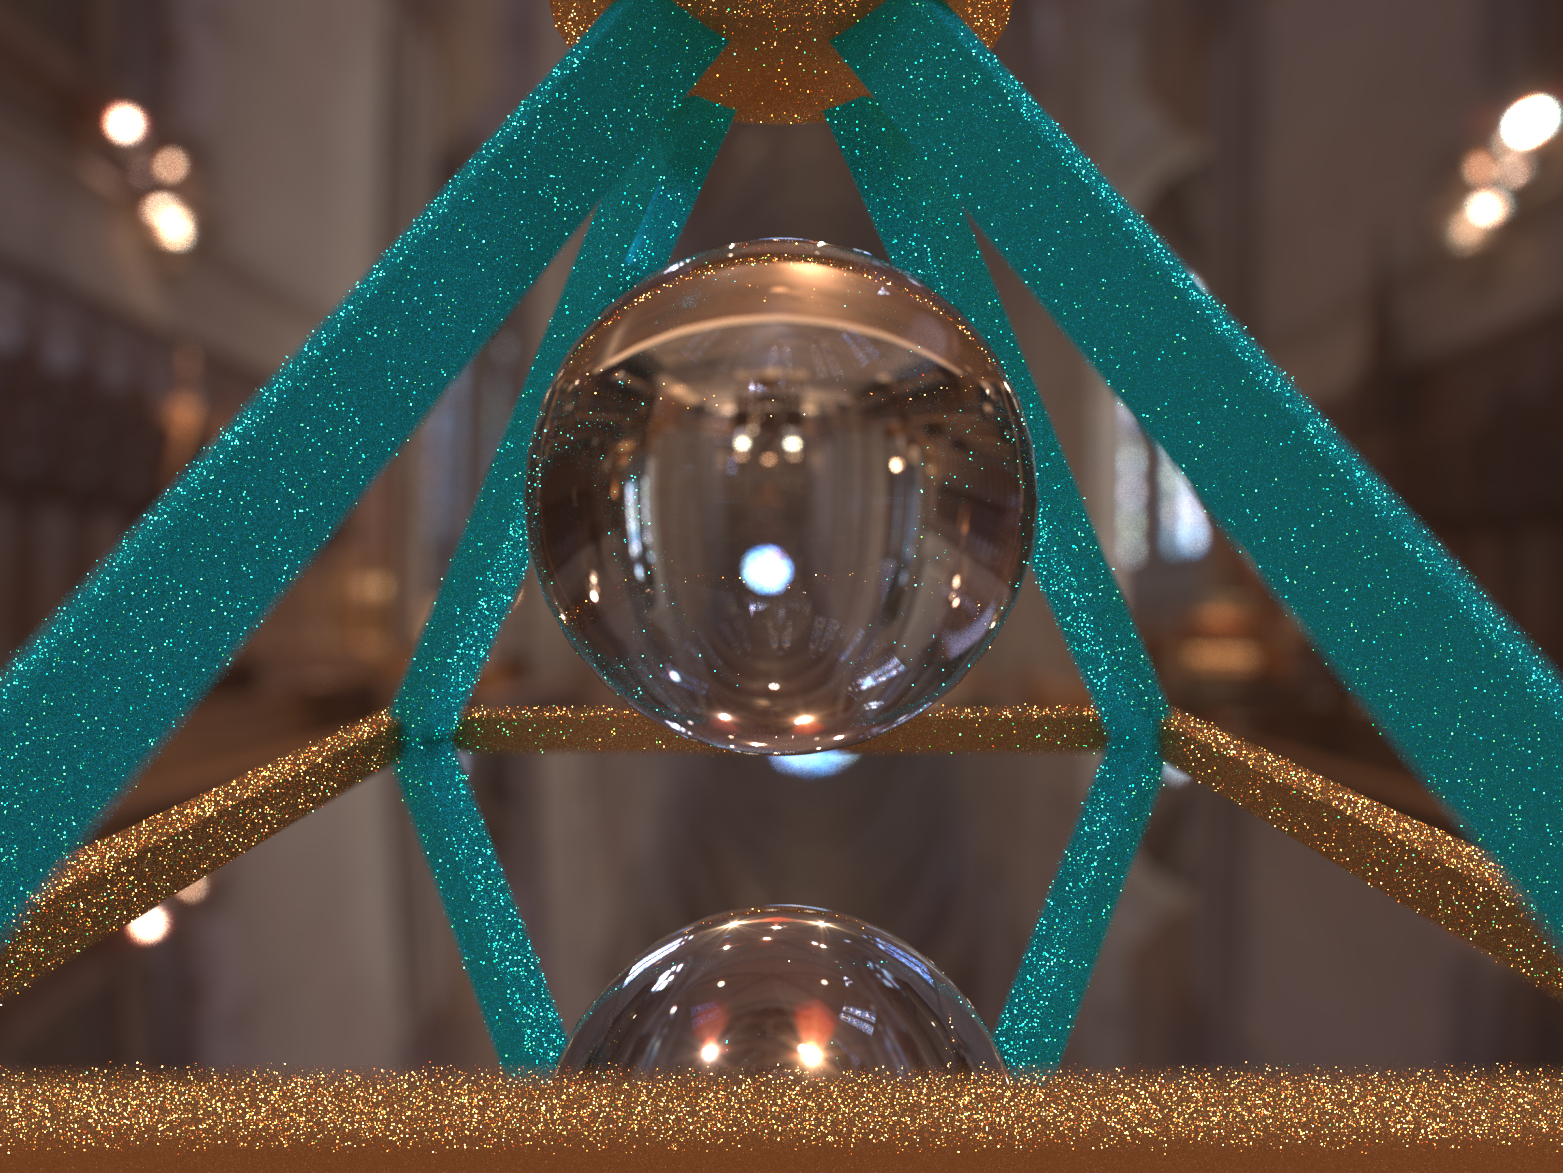
\includegraphics[width=1\linewidth]{images/escena_2400x1800_128spp_dof20-03_screencap.png}
%\caption{Render con DoF: Distancia focal: 20, Radio lente: 0.3}
%\label{fig:disp}
%\end{figure}
\begin{figure}[h]
\centering
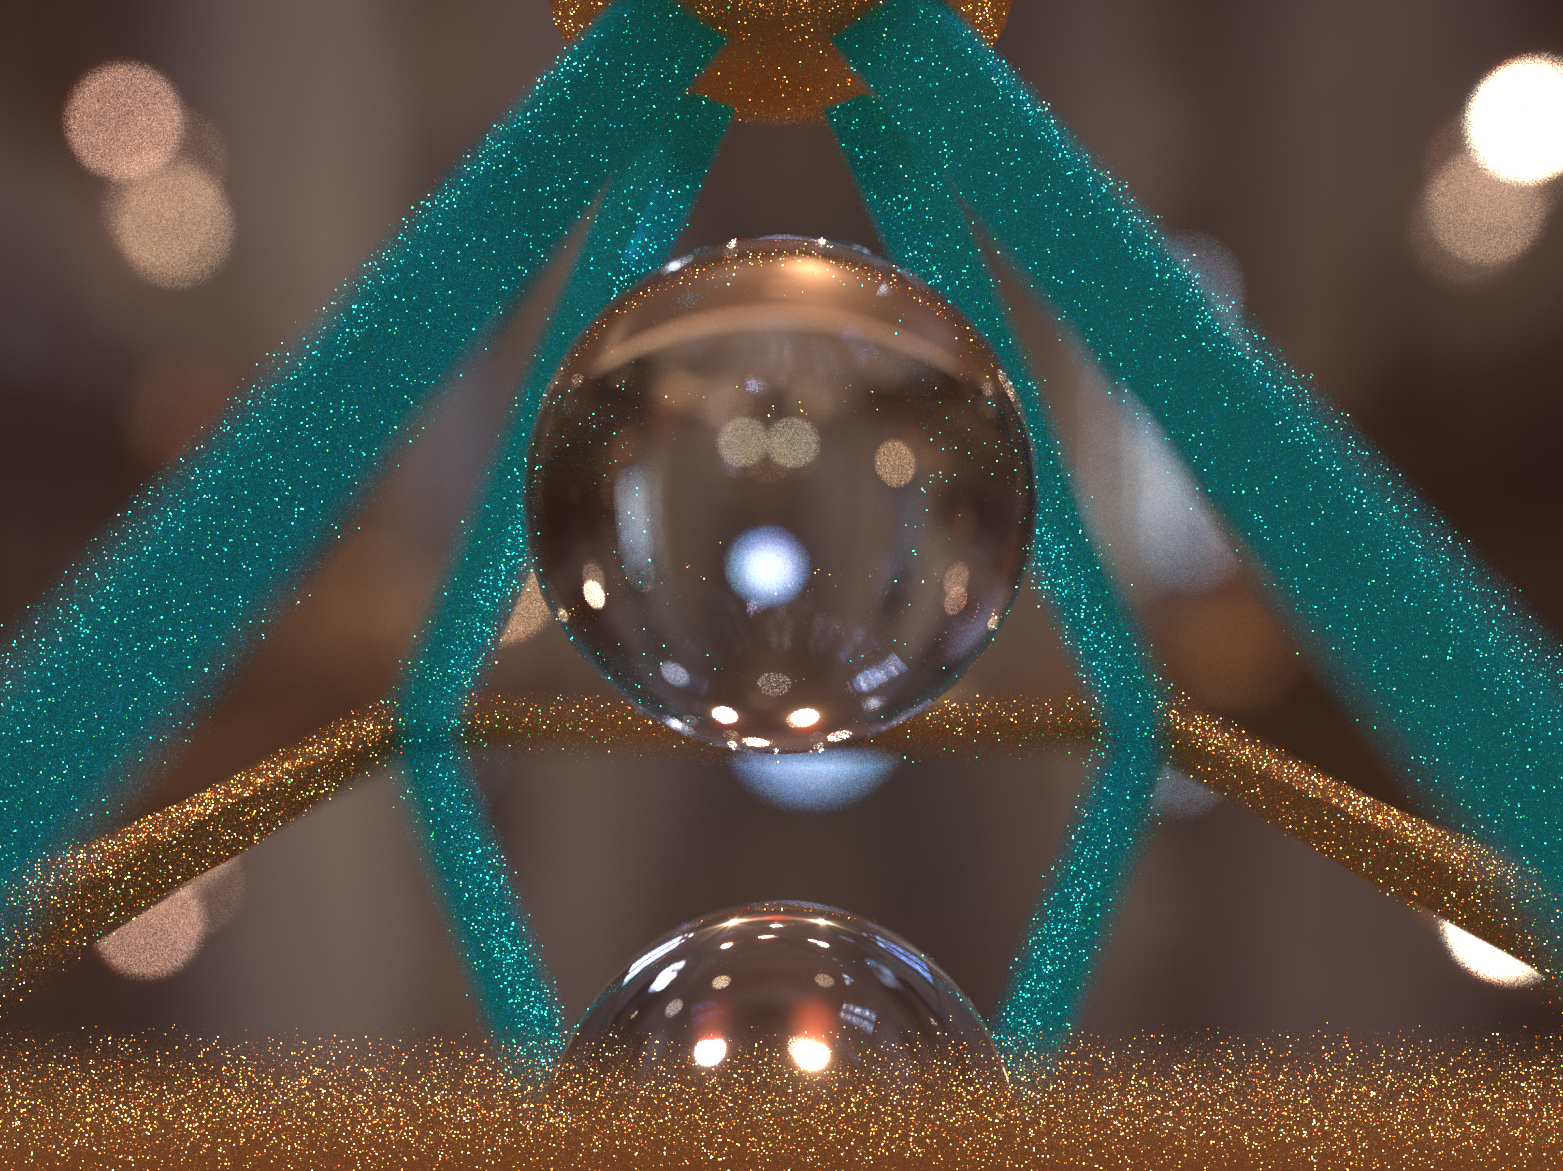
\includegraphics[width=1\linewidth]{images/escena_2400x1800_128spp_dof20-1_screencap.png}
\caption{Render con DoF: Distancia focal 20:, Radio lente: 1}
\label{fig:disp}
\end{figure}

Por último, actualizamos el rayo tomando como punto de inicio el punto muestreado sobre la lente, multiplicado este por la matriz de cámara, y como nueva dirección utilizamos el vector que une el origen del nuevo rayo y el punto de enfoque.\\

Los parámetros de \emph{Depth of Field} se han expuesto en la configuración de escena como parámetros de la cámara llamados \emph{focalDistance} y \emph{lensRadius}, definiendo la distancia focal y el radio de la lente (o apertura), respectivamente. Estos parámetros son de tipo float. Es interesante resaltar que a menor radio de la lente menor sera el efecto producido por el \textit{Depth of Field}, ya que el area de los círculos de confusión de los puntos fuera del plano de enfoque serán menores, ya que mientras más pequeña sea esa lente más nos estaremos acercando a la camara \textit{pin-hole} ideal con apertura infinitamente pequeña.

\newpage

\section{Environment Map Lighting}
Para implementar el \emph{Environment Map Lighting} se ha consultado la documentación disponible de \emph{Mitsuba} y la tercera edición de \emph{Physically Based Rendering}. De \emph{Mitsuba} se han extraído las ecuaciones de conversión de coordenadas esféricas a coordenadas de textura, y de \emph{Physically Based Rendering} se ha obtenido el algoritmo base para muestrear una proyección esférica a partir de un rayo. Para poder implementar los mapas de entorno ha sido necesario además un \emph{Light Map} que se ha descargado de la web de la \emph{University of Southern California} ( http://gl.ict.usc.edu/Data/HighResProbes/ ), concretamente el mapa de entorno de la Grace Cathedral de San Francisco, California.\\

Debido a que el entorno se considera una esfera de dimensiones infinitas, esta es muestreada cuando el rayo no interseca con la geometría de la escena. En \emph{Nori}, cuando esto ocurre, es equivalente a una intersección con el fondo de la escena. Por tanto la implementación se ha realizado en la función \emph{getBackground()} de la escena (\emph{scene.cpp}), que es llamada cuando el rayo no ha intersecado con ninguna geometría. Esta función únicamente hará una llamada a la clase \emph{Environment} pasando como argumento el rayo en cuestión, que es una clase que define un \emph{emitter} y que se explica a continuación.\\

Al necesitarse únicamente una componente emisiva y al tratarse el mapa de entorno como una luz de área, solamente es necesario evaluar el valor correspondiente al texel de la intersección rayo-esfera. Por simplicidad no hemos implementado ningún filtrado, por lo que accederemos al pixel más cercano en la textura. Esto ocurre en la clase \emph{Environment}, que es una clase que extiende de \emph{Emitter} y almacena un \emph{Bitmap} correspondiente a la textura definida como parámetro del \emph{emitter}. El método \emph{eval()} de esta clase recibirá un rayo y devolverá el color del pixel correspondiente del \emph{environvent map}. Para ello primero se realiza una conversión de un vector (el rayo en coordenadas del mundo) a coordenadas esféricas. Al tratarse de una esfera de radio infinito, siempre estará centrada y no será necesario hacer ninguna transformación sobre el rayo. Por tanto la conversión de vector a coordenadas esféricas será simplemente:

\begin{gather}
\theta = \arccos{y}\\
\varphi =  \arctan{\frac{x}{-z}}
\end{gather}

A partir de las coordenadas polares, y sabiendo que $\varphi$ está representado en el dominio de $2\pi$ y que $\theta$ se representa en el dominio de $\pi$, sólo es necesario multiplicar las coordenadas por la inversa de $2\pi$ y de $\pi$ respectivamente para obtener las coordenadas de textura. Estos valores están definidos como constantes en \emph{Nori} como \emph{INV\_TWOPI} e \emph{INV\_PI}.\\

Ahora, teniendo ya las coordenadas de textura normalizadas, estas se transforman en un valor entre $0$ y $n-1$, donde $n$ es el número de pixels de la imagen en la coordenada correspondiente. Este valor puede corresponder a un punto fuera de la textura, siendo necesario tratar estos casos límite, para lo que se ha definido el comportamiento de \emph{repeat} en el eje x y de \emph{clamp} en el eje y. El efecto \emph{repeat} se consigue calculando el \emph{modulo} (resto) de la coordenada x respecto al máximo de pixels en el eje x, mientras que el efecto \emph{clamp} se ha conseguido simplemente limitando los valores entre $0$ y $n-1$.\\

El resultado es que dado un rayo, se obtienen las coordenadas del pixel más cercano correspondiente a la intersección con la esfera que define la \emph{Light Probe}, tomándose su valor como la radianza en ese punto de la esfera.

\newpage
\section{Otros efectos}
Además de los efectos añadidos para esta entrega, se ha hecho uso de los efectos implementados en entregas previas. Para demostrarlo, se han renderizado dos versiones finales de la imagen, uno mediante el uso de una esfera reflectiva perfecta (equivalente a la imagen motivacional) y otro mediante el uso de una esfera dieléctrica. Las dos imágenes pueden verse al final del documento, en la sección de resultados.\\

También se emplean otras técnicas implementadas en anteriores entregas, como la de ruleta rusa.

\section{Dificultades encontradas}
Principalmente las dificultades se han encontrado a la hora de implementar los \emph{Environment Maps}. Aunque la información estaba disponible en los recursos habituales, llegar a filtrar la información útil ha sido complicado y ha sido necesario reimplementar un mismo algoritmo de varias formas diferentes hasta conseguir los resultados esperados. \\

Tampoco ha sido posible implementar optimizaciones extra, como puede ser muestreo por importancia o \emph{Next Event Estimation}, ya que para ello era necesario realizar un pre-procesado de la \emph{Light Probe} que añadía complejidad excesiva a la implementación. Por este motivo las superficies difusas de nuestros resultados muestran ruido.\\

Además hemos dado con un problema derivado de la implementación del operador modulo (\%) en C++, que no se comporta como el operador modulo matemático cuando se calcula el modulo de valores negativos, y que hasta descubrir que estaba devolviendo valores negativos que afectaban a los resultados, nos ha dado muchos quebraderos de cabeza.

\newpage
\section{Resultados finales}
Como se mencionaba previamente, dado que la imagen motivacional utiliza una esfera que actúa como un espejo perfecto, para poder mostrar también el efecto de materiales dieléctricos se ha renderizado la escena cambiando la esfera central por un material dieléctrico, mostrándose ambos resultados. Además se ha optado por renderizar los ``soportes'' como materiales difusos de color similar al de la imagen motivacional, ya que es el comportamiento más cercano al original que podemos representar en nuestro motor, mientras que la base del soporte, al no disponer de materiales glossy, se ha modelado con un material de espejo perfecto. Todo el modelado se ha realizado en 3DSMax.\\

Como resultado final tenemos un render que representa fielmente la reflexión y refracción de los rayos de luz, pero que a falta de optimizaciones en el muestreo de la textura del environment map muestra niveles altos de ruido en las superficies difusas. Creemos que este ruido podría disminuirse en gran medida o incluso eliminarse en caso de utilizar técnicas que muestreen correctamente los puntos de mayor iluminación de la textura del entorno.

\begin{figure}[h]
\centering
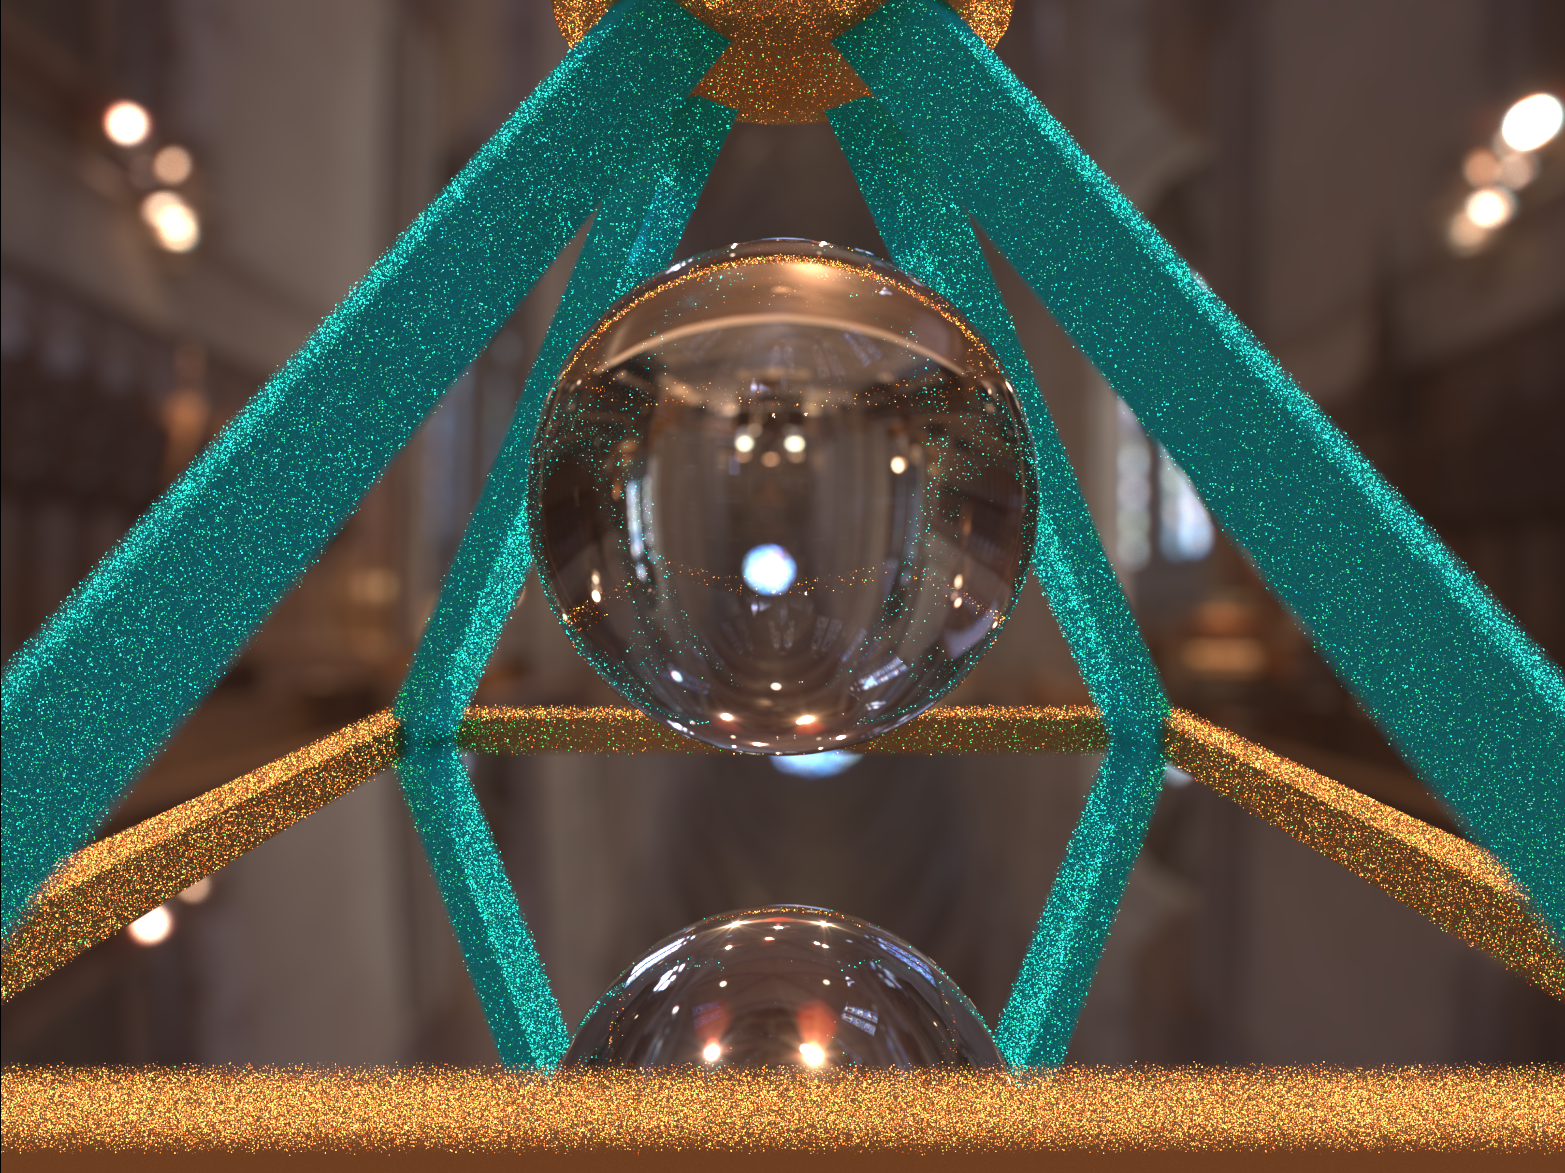
\includegraphics[width=1\linewidth]{images/escena_2400x1800_2048spp_dof20-03_screencap.png}
\caption{Esfera dieléctrica - 2400x1800 2048spp - Distancia focal: 20, Radio lente: 0.3}
\label{fig:disp}
\end{figure}

\begin{figure}[h]
\centering
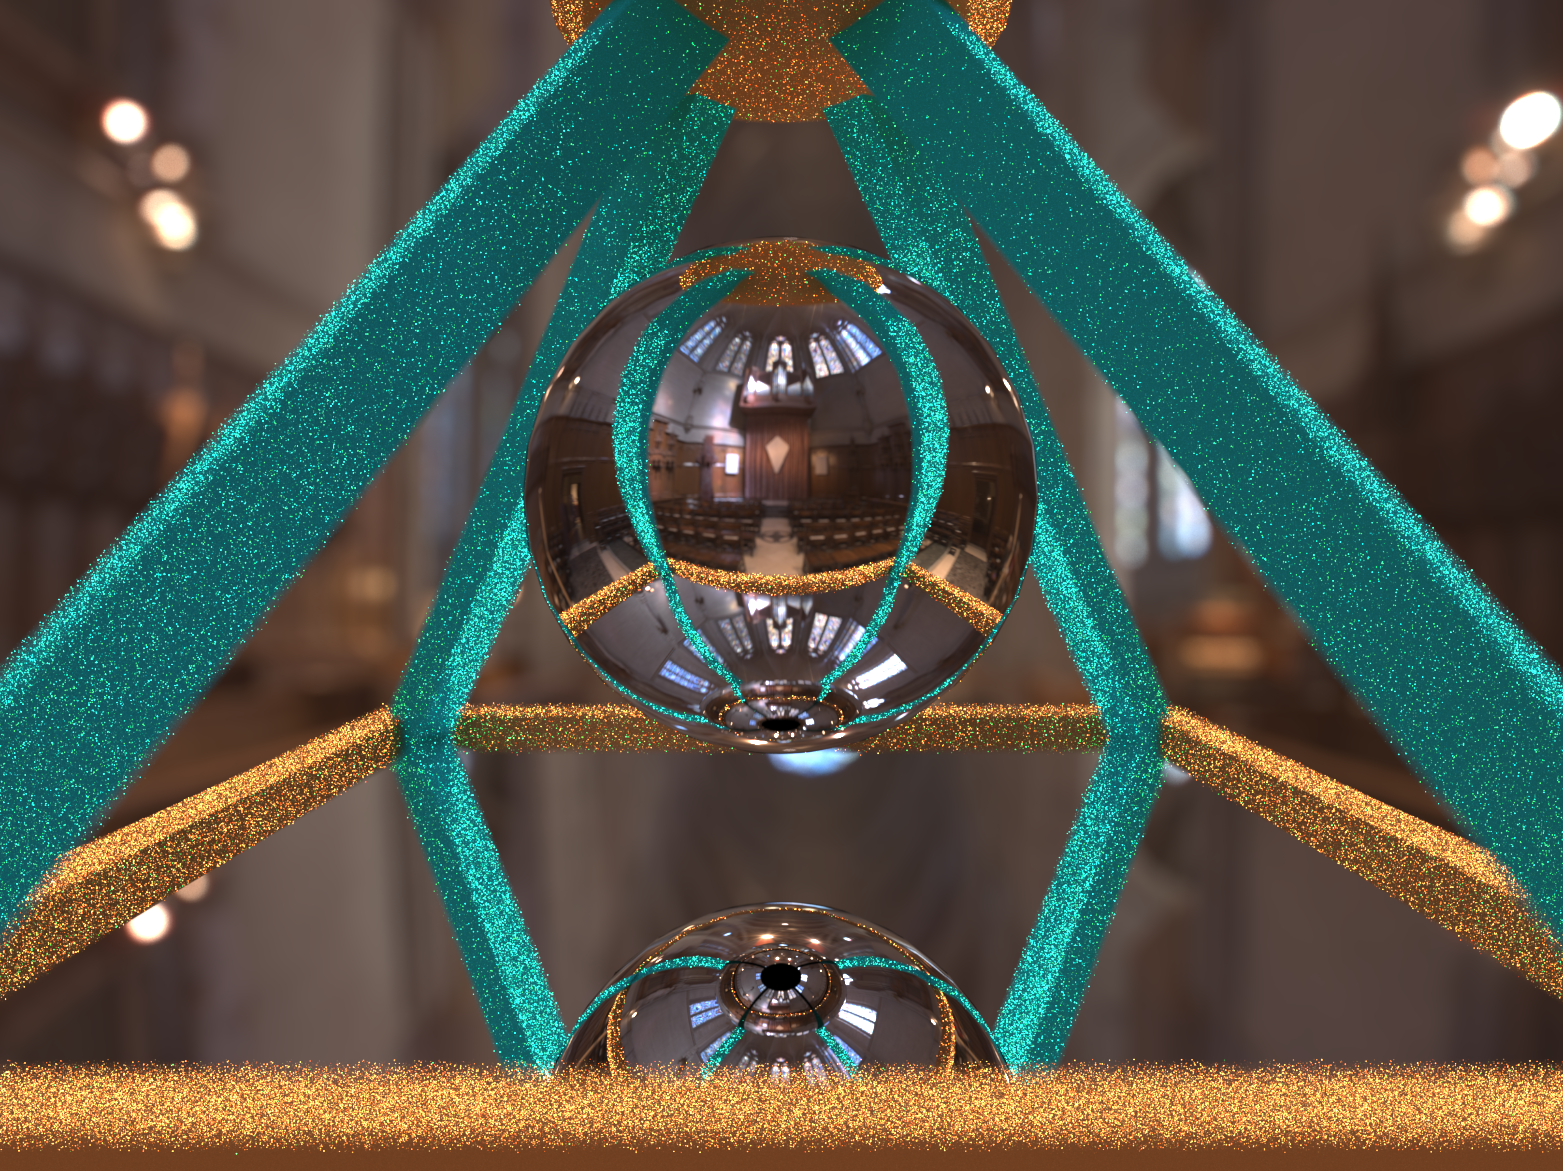
\includegraphics[width=1\linewidth]{images/escenamirror_2400x1800_2048spp_dof20-03_screencap.png}
\caption{Esfera espejo - 2400x1800 2048spp - Distancia focal: 20, Radio lente: 0.3}
\label{fig:disp}
\end{figure}
\end{document}